\documentclass[12pt, oneside]{article}
\usepackage[utf8]{inputenc}
\usepackage{polski}
\renewcommand*{\figurename}{Rys.}
\usepackage{graphicx}
\usepackage{float}
\usepackage{geometry}
\usepackage{subcaption}
\usepackage{indentfirst}
\usepackage{fancyvrb}
\setlength{\parindent}{4em}
\setlength{\parskip}{1em}
\geometry{
	left=25mm,
	right=25mm,%
	bindingoffset=10mm, 
	top=25mm, 
	bottom=25mm}
\title{
	Eksploracja danych \\
	Światowy program szczepień przeciwko COVID-19
}
\author{
	Marek Grudkowski 156587
	\\
	Kamil Kaczmarkiewicz 171701
}

\begin{document}

\maketitle

\section{Ogólny opis danych}

Zbiór danych dotyczy aktualnego postępu poszczególnych państw w szczepieniach przeciwko COVID-19. Zawiera on informacje pochodzące prawie ze wszystkich krajów na świecie podzielone na poszczególne dni. Program szczepień przeciwko COVID to w dobie pandemii niezwykle gorący temat. Naszym zdaniem warto się na nim skupić, gdyż może zawierać wiele ukrytych informacji, które mogą przydać się w walce z pandemią i przyspieszyć sam proces szczepień. 

\section{Cel eksploracji i kryteria sukcesu}

Celem eksploracji danych jest zgłębienie wszelkich tajemnic ukrytych w analizowanym zbiorze danych. Takie informacje można wykorzystać do wskazania zarówno państw, które najlepiej przeprowadzają program szczepień, jak i tych w których proces ten przebiega bardzo słabo. Dzięki temu niektóre państwa mogłyby się wzorować na tych , które radzą sobie najlepiej oraz uniknąć błędów, jakie popełniły te, które są najgorsze w rankingu. Dodatkowym celem może być predykcja zapotrzebowania szczepionek w danych krajach na najbliższe miesiące, która mogłaby by zapobiec marnowaniu się dawek oraz pozwolić rządom na świecie lepiej zaplanować \textit{zakupy} oraz logistykę akcji na terenie swojego kraju.  Jako ostatni cel można uznać wskazanie prawdopodobnej daty zakończenia światowego programu szczepień. 
\par
Jako kryteria sukcesu eksploracji danych można uznać odpowiednio wysoką (przykładowo $80$ \%) zgodność predykcji wykonywanych szczepień w danych państwach z rzeczywistymi danymi, które są aktualizowane na bieżąco. 

\newpage

\section{Charakterystyka zbioru danych}
Zbiór danych na stan dnia pisania tego sprawozdania zawiera ponad 13300 przykładów. Dane aktualizowane są zazwyczaj co kilka dni i pochodzą z wielu różnych źródeł. Zazwyczaj są nimi organy krajowe lub lokalne, czy międzynarodowe organizacje. Dla każdego przykładu podane jest źródło i jego adres internetowy, co daje możliwość weryfikacji w przypadku jakichkolwiek wątpliwości co do poprawności danych. Dane zapisane są w jednym pliku w formacie csv i podzielone są na następujące kolumny:

\paragraph{country}
\mbox{}\\
Nazwa państwa lub regionu, którego dotyczy dany przykład.

\paragraph{ISO code}
\mbox{}\\
Trzyliterowy kod państwa zgodny z normą ISO $3166-1$

\paragraph{date}
\mbox{}\\
Data pozyskania danych. 

\paragraph{total vaccinations}
\mbox{}\\
Całkowita liczba podanych dawek. Zliczane są tutaj pojedyncze dawki i nie mogą być równe całkowitej liczbie zaszczepionych osób, w zależności od schematu dawkowania np. jedna osoba może przyjąć kilka dawek.

\paragraph{total vaccinations per hundred}
\mbox{}\\
Całkowita liczba podanych dawek szczepionki w przeliczeniu na sto osób w liczbie ludności całego kraju.

\paragraph{daily vaccinations raw}
\mbox{}\\
Dzienna zmiana w całkowitej liczbie podanych dawek. Oblicza się ją tylko dla kolejnych dni. Surowy środek w celu kontroli danych i jej przejrzystości. Autorzy zestawu nie zalecają korzystania z tego atrybutu. 

\paragraph{daily vaccinations}
\mbox{}\\
Liczba dawek podawanych dziennie. Liczba ta jest wygładzana w ujęciu 7 dni. W przypadku krajów, które nie przekazują danych w ujęciu dziennym zakłada się, że dawki zmieniały się jednakowo we wszystkich okresach, w których nie przekazywano danych. Tak wypełnione dane uśrednia się dodatkowo w 7 dniowym oknie.

\paragraph{daily vaccinations per million}
\mbox{}\\
Liczba dawek podawanych dziennie w przeliczeniu na milion osób w ludności całego kraju

\paragraph{people vaccinated}
\mbox{}\\
Całkowita liczba osób, które otrzymały przynajmniej jedną dawkę szczepionki. Jeśli osoba otrzyma pierwszą dawkę liczba zwiększana jest jeden, jeśli otrzyma drugą, pozostaje taka sama. 

\paragraph{people vaccinated per hundred}
\mbox{}\\
Całkowita liczba osób, które otrzymały przynajmniej jedną dawkę szczepionki w przeliczeniu na sto osób w liczbie ludności całego kraju.

\paragraph{people fully vaccinated}
\mbox{}\\
Całkowita liczba osób, które otrzymały wszystkie dawki zgodnie ze schematem szczepienia. Jeśli bierzemy pod uwagę schemat szczepień z dwoma dawkami - przy pierwszej dawce liczba nie zmienia się, po drugiej dawce zwiększana jest o 1. 

\paragraph{people fully vaccinated per hundred}
\mbox{}\\
Całkowita liczba osób, które otrzymały wszystkie dawki zgodnie ze schematem szczepienia w przeliczeniu na sto osób w liczbie ludności całego kraju.

\paragraph{source name}
\mbox{}\\
Nazwa źródła, z którego pochodzą dane.

\paragraph{source website}
\mbox{}\\
Strona internetowa, źródła z którego pochodzą dane. 



\section{Eksploracyjna analiza danych}


\subsection{Atrybuty nominalne}

\paragraph{country oraz ISO code}
\mbox{}\\
Są to pierwsze analizowane atrybuty. Zgodnie z normą ISO 3166 kody państw powinny być trzyliterowe. Sprawdziliśmy to i część przykładów nie spełniała tego warunku. Państwa, które posiadają inny niż trzyliterowy kod ISO:
\begin{verbatim}
England has code OWID_ENG
Kosovo has code OWID_KOS
Northern Cyprus has code OWID_CYN
Northern Ireland has code OWID_NIR
Scotland has code OWID_SCT
Wales has code OWID_WLS
\end{verbatim}
Zgodnie z opisem dostarczonym przez twórców zbioru nie jest to błąd, lecz skutek pozyskiwania danych z różnych źródeł. Dla każdego z niepoprawnych kodów można przydzielić jego poprawny odpowiednik.

Wartość kodu dla Kosowa według danych na oficjalnych stronach organizacji ISO powinno mieć kod \textit{XKX}. Północny Cypr powinien zostać włączony do Cypru, a pozostałe regiony (Anglia, Walia, Irlandia Północna oraz Walia) powinny zostać wcielone do  Wielkiej Brytanii. Podczas przygotowywania tych atrybutów kluczowe jest połączenie przykładów z kilku regionów w jeden przykład, jeśli dotyczą one tej samej daty. 


Liczebność przykładów podzielonych na państwa można zaprezentować w postaci histogramu i wykresu pudełkowego. Pozwolą one zauważyć, które z państw dostarczyły mało danych, a które zapewniły ich odpowiednio dużo. Wyniki zamieszczone są na wykresach poniżej (Rysunek nr \ref{Rys:histogramSamples}, \ref{Rys:boxplotSamples})

\begin{figure}[h]
\centering
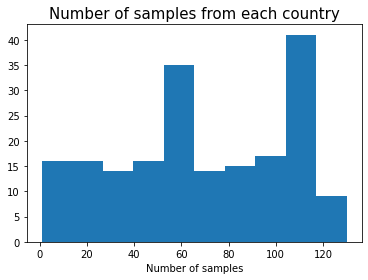
\includegraphics[width=0.6\textwidth]{../img/number_of_samples.png} 
\caption{Liczba przykładów dostarczonych przez poszczególne państwa (histogram)}
\label{Rys:histogramSamples}
\end{figure}

\begin{figure}[h]
\centering
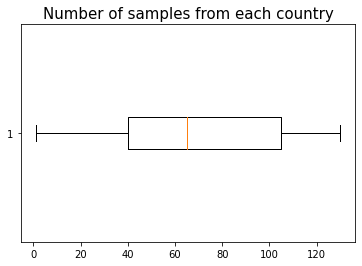
\includegraphics[width=0.6\textwidth]{../img/boxplot_of_samples.png} 
\caption{Liczba przykładów dostarczonych przez poszczególne państwa (pudełkowy)}
\label{Rys:boxplotSamples}
\end{figure}






\subsection{Atrybuty numeryczne}

Pierwszym krokiem w analizie atrybutów numerycznych jest sprawdzenie, w jakiej liczbie występują braki w każdej kolumnie. Wyniki operacji sprawdzającej ten fakt, poniżej:

\begin{verbatim}
Size of data is: (13307, 13)
Missing values in dataset: 
country                                   0
iso_code                                  0
date                                      0
total_vaccinations                     5255
people_vaccinated                      5931
people_fully_vaccinated                7926
daily_vaccinations_raw                 6529
daily_vaccinations                      220
total_vaccinations_per_hundred         5255
people_vaccinated_per_hundred          5931
people_fully_vaccinated_per_hundred    7926
daily_vaccinations_per_million          220
vaccines                                  0
\end{verbatim}

Niestety jak widać są to bardzo duże braki, którymi należy się zająć w późniejszym etapie. Na pierwszy rzut oka widać, że atrybuty łączą się w pary pod dwoma względami: nazwą oraz liczbą brakujących wartości. Zgodnie z opisem danych dostarczonym przez autorów w takiej parze jeden z atrybutów jest zależny od drugiego i pokazuje daną wartość w stosunku do populacji danego kraju. Aby upewnić się można sporządzić wykres prezentujący wartość korelacji pomiędzy poszczególnymi atrybutami (Rysunek \ref{Rys:corrHeatMapWorld})

Nie widać na nim zależności o których wspomnieli autorzy. Przyczyną jest liczenie korelacji dla całego zbioru danych, a nie konkretnego państwa. Jeśli do funkcji rysującej wykres przekażemy tylko zakres  obejmujący jedno państwo totalnie zmienia on swój wygląd. Przykładowy wykres dla USA można zobaczyć na rysunku nr \ref{Rys:corrHeatMapUsa}.


\begin{figure}[!ht]

\centering
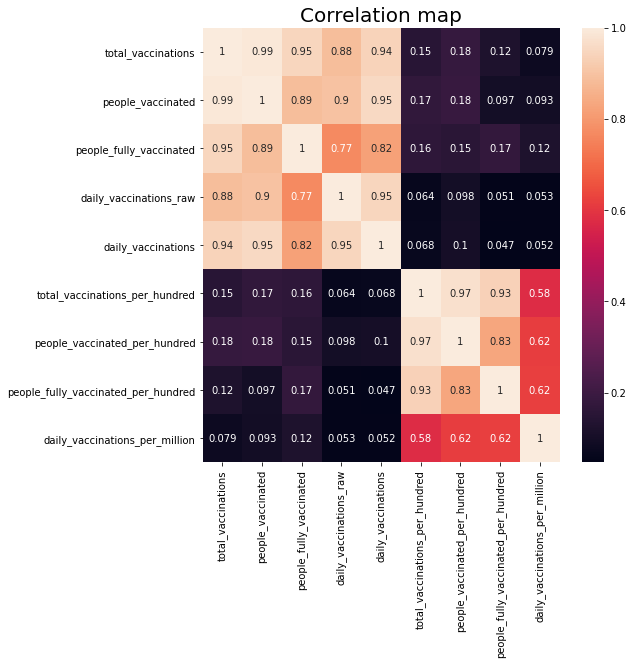
\includegraphics[scale=0.45]{../img/corelation.png} 
\caption{Korelacja pomiędzy atrybutami całego zbioru danych\label{Rys:corrHeatMapWorld}}

\centering
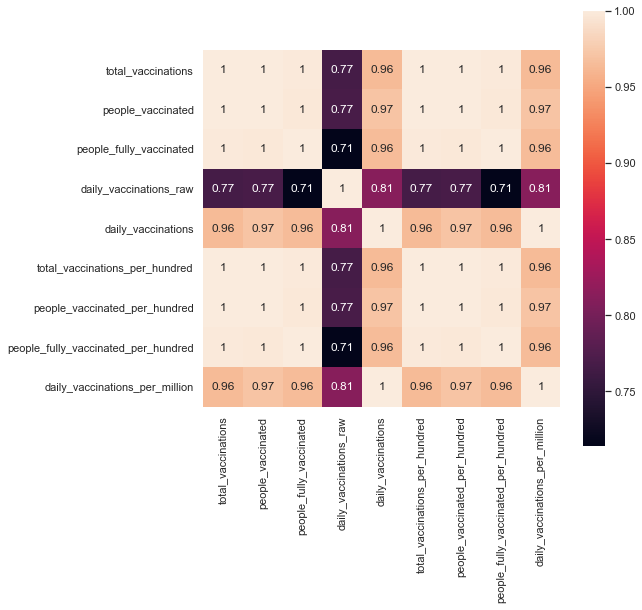
\includegraphics[scale=0.45]{../img/usa_corr.png} 
\caption{Korelacja pomiędzy atrybutami zbioru danych dla USA}
\label{Rys:corrHeatMapUsa}

\end{figure}




\newpage
Aby upewnić się, czy dla wszystkich państw występuje opisana zależność, można osobno dla każdego państwa obliczyć korelację pomiędzy atrybutami i sporządzić histogram, na którym role pojedynczych próbek będą pełnić państwa (Rysunek \ref{Rys:histOfCorrAttr}). Zdecydowanie widać, że na każdym z owych wykresów niemal 100\% próbek wskazywało na korelację równą 1, co oznacza zgodność z tym, co napisali autorzy zestawu danych. Owe powiązania między atrybutami można opisać w postaci zależności:

\begin{Verbatim}[tabsize=4]
TotalVaccinationsPerHundred = 
	TotalVaccinations / CountryPopulation * 100
PeopleVaccinatedPerHundred = 
	PeopleVaccinated / CountryPopulation * 100
PeopleFullyVaccinatedPerHundred = 
	PeopleFullyVaccinated / CountryPopulation * 100
DailyVaccinationsPerMillion = 
	DailyVaccinations / CountryPopulation * 1 000 000
\end{Verbatim}




\begin{figure}[!ht]
  \begin{subfigure}[t]{.45\textwidth}
    \centering
    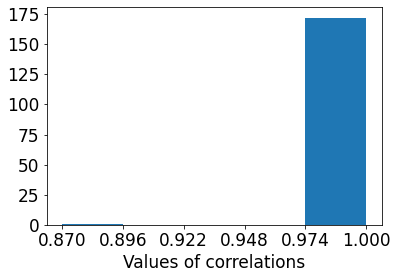
\includegraphics[width=\linewidth]{../img/null_column_diff1.png}
    \caption{Korelacja między dzienną liczbą wykonanych szczepień ogółem i na milion osób}
  \end{subfigure}
  \hfill
  \begin{subfigure}[t]{.45\textwidth}
    \centering
    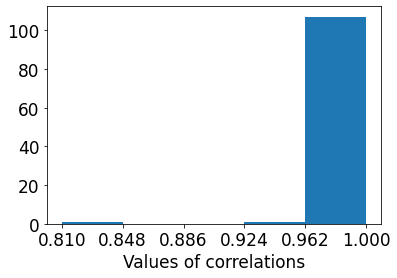
\includegraphics[width=\linewidth]{../img/null_column_diff2.png}
    \caption{Korelacja między liczbą ludzi w pełni zaszczepionymi ogółem i na 100 osób}
  \end{subfigure}

  \begin{subfigure}[t]{.45\textwidth}
    \centering
    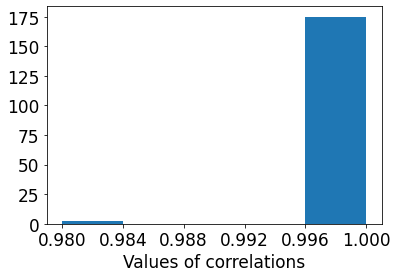
\includegraphics[width=\linewidth]{../img/null_column_diff3.png}
    \caption{Korelacja między liczbą ludzi którzy przyjęli choć jedną dawkę ogółem i na 100 osób}
  \end{subfigure}
  \hfill
  \begin{subfigure}[t]{.45\textwidth}
    \centering
    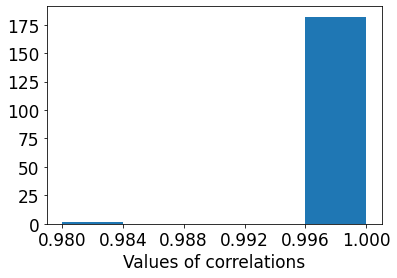
\includegraphics[width=\linewidth]{../img/null_column_diff4.png}
    \caption{Korelacja między liczbą wykonanych szczepień ogółem i na sto osób}
  \end{subfigure}
  \caption{Korelacje pomiędzy poszczególnym atrybutami zbioru}
\label{Rys:histOfCorrAttr}
\end{figure}


Jedynym atrybutem który pozostał bez pary jest \textit{daily\_vaccinations\_raw}. Jednakże wedle zaleczeń autorów zestawu nie powinien być uwzględniany podczas analizy, dlatego można z niego zrezygnować. 

Część z brakujących wpisów można łatwo uzupełnić, wykorzystując opisane wcześniej reguły. Łączną sumę podanych dawek szczepionki można wyznaczyć prostą metodą, jeśli założymy liniową progresją pomiędzy odległymi wartościami. Pozwoli to wypełnić nie tylko jedną kolumnę, ale aż dwie - przecież liczba podanych dawek na sto osób, to ta sama wartość, tylko zmieniona na podstawie populacji w danym kraju.  Podobne założenia można przyjąć w przypadku liczby osób, które przyjęły choć jedną dawkę, liczby osób w pełni uodpornionych oraz ich względnych odpowiednikach.


Te trzy pary atrybutów to wielkości rosnące w czasie i pod uwagę powinna być brana najnowsza wartość, osobno dla każdego kraju. Używanie do wizualizacji atrybutów bezwzględnych nie jest dobrym pomysłem, gdyż taki wykres będzie pokazywał jedynie zależności w liczbie mieszkańców danych krajów. Najlepszym rozwiązaniem by pokazać sprawność programu szczepień w danym państwie jest więc sporządzenie wykresów pudełkowych dla atrybutów względnych (Rysunek \ref{Rys:boxTotalVacc}, \ref{Rys:boxPeopleVacc} i \ref{Rys:boxFullyVacc})


\paragraph{Total vaccinations per hundred}
\mbox{}\\

Na wykresie widać, że aktualnie w większości krajów liczba wykonanych szczepień na sto osób nie przekracza 50. Poza zakresem wąsów można zauważyć też kilkanaście skrajnych wartości. Zapewne są to kraje przodujące w programie szczepień. Najbardziej skrajny punkt dotyczy Gibraltaru. Jest to małe państwo, które liczy około 35 tysięcy mieszkańców. Bardzo szybko zrealizowali program szczepień, gdyż przed końcem marca każdy mieszkaniec po 16 roku życia otrzymał drugą dawkę. 
\begin{figure}[!ht]
\centering
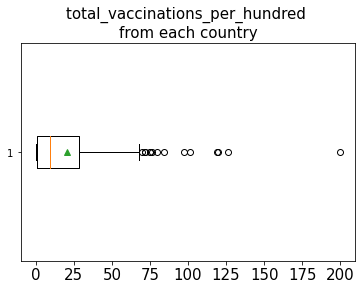
\includegraphics[scale=0.5]{../img/box_total_vaccinations.png} 
\caption{Rozkład liczby wykonanych szczepień}
\label{Rys:boxTotalVacc}
\end{figure}

\newpage

\paragraph{People vaccinated per hundred}
\mbox{}\\
\begin{figure}[!ht]
\centering
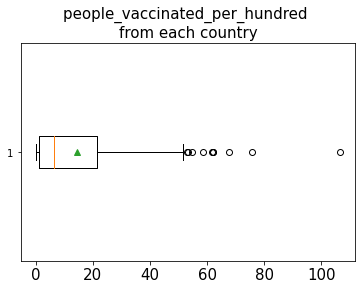
\includegraphics[scale=0.5]{../img/box_people_vaccinated.png} 
\caption{Rozkład liczby zaszczepionych osób}
\label{Rys:boxPeopleVacc}
\end{figure}

W przypadku liczby osób, którym podano szczepionkę sytuacja wygląda bardzo podobnie. Tutaj również bardzo wyróżnia się Gibraltar, który o dziwo zaszczepił aż 106 osób na 100 obywateli swojego kraju. Bardzo możliwe, że nastąpił tutaj błąd przy wprowadzaniu danych, gdyż na wykresie dotyczącym osób w pełni zaszczepionych Gibraltar opisuje liczba 93. Wiedząc, że wszystkich obywateli zaszczepiono tam dwiema dawkami - można porównać te dwie wielkości. Po krótkich obliczeniach można stwierdzić, że te 106 osób to tak naprawdę 100, a te nadwyżkowe 6 to osoby które otrzymywały drugą dawkę szczepionki. 


\paragraph{People fully vaccinated per hundred}
\mbox{}\\
\begin{figure}[h]
\centering
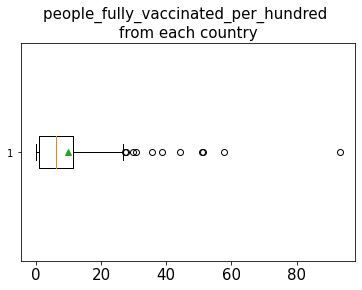
\includegraphics[scale=0.5]{../img/box_fully_vaccinated.png} 
\caption{Rozkład liczby w pełni zaszczepionych osób}
\label{Rys:boxFullyVacc}
\end{figure}

\newpage

\paragraph{Daily vaccinations}
\mbox{}\\

W porównaniu do tych 3 miar, inaczej wygląda sytuacja w przypadku dziennej ilości podanych dawek. Według autorów zbioru danych jest to atrybut, który obliczają sami na podstawie publikowanej przez rządy liczby wykonanych szczepień. Jako, że takie informacje nie są publikowane codzienne występuje  właśnie potrzeba obliczania dziennej ilości podanych dawek. Wylicza się to w trzech krokach na podstawie opublikowanej liczby wykonanych szczepień:
\begin{enumerate}
\item Za pomocą interpolacji uzupełnia się brakujące wartości totalnej liczby wykonanych szczepień
\item Na podstawie różnicy z dniem poprzednim wylicza się ilość podanych w danym dniu dawek
\item Taka wyliczona liczba jest ostatecznie uśredniana z wartością jaka występuje w ciągu ostatniego tygodnia 
\end{enumerate}




%Pierwszym atrybutem, w którym łatwo można uzupełnić dane jest \textit{total\_vaccinations}. Dotyczy on łącznej sumy wykonanych szczepień w danym państwie. W przypadku brakujących wartości można je wypełnić zakładając idealną liniową progresję pomiędzy odległymi wartościami.

%Po wypełnieniu kolumny z totalną liczbą podanych dawek, można łatwo uzupełnić kolumnę opisującą średnią liczbę podanych dawek na sto osób. Wystarczy dla brakujących wartości wstawić liczbę opisaną zależnością:
%\begin{verbatim}
%liczbaPodanychDawekNaSto = totalnaLiczbaPodanychDawek / ludnoscKraju * 100 
%\end{verbatim}

%Aby to zrobić najpierw potrzebna jest liczba ludności w danym kraju. Aby wykorzystać w pełni nasz zbiór danych wielkość tą obliczyliśmy dla każdego państwa na podstawie średniego ilorazu liczby podanych dawek oraz liczby podanych dawek na sto osób, przy czym tutaj braliśmy pod uwagę tylko przykłady, w których nie brakowało żadnych wartości. Ostatecznie po wypełnieniu tych atrybutów liczba brakujących danych wygląda następująco:



\section{Wnioski i podsumowanie}

Widać dużą rozbieżność między liczbą dostarczonych próbek przez państwa. Zapewne ma to związek z tym, że część z państw nie rozpoczęła w ogóle programu szczepień. Przykładowe państwa, które dostarczyły skrajne liczby przykładów poniżej:
\begin{verbatim}
Canada has delivered 130 samples
China has delivered 129 samples
Russia has delivered 129 samples
Israel has delivered 125 samples
United States has delivered 124 samples
Djibouti has delivered only 1 samples
Ethiopia has delivered only 1 samples
Libya has delivered only 1 samples
Somalia has delivered only 1 samples
Timor has delivered only 1 samples
\end{verbatim}

Dużym problemem są też bardzo duże braki w danych. Przed rozpoczęciem pracy ze zbiorem trzeba będzie poświęcić dużo pracy, aby uzupełnić wszystkie braki i zestandaryzować cały zbiór. Na część z nich odpowiedź na pytanie \textit{co tam powinno być} jest w miarę prosta. Jednak w przypadku takich atrybutów jak liczba osób w pełni zaszczepionych może być ciężko go wypełnić. 

\begin{verbatim}
Missing values in dataset: 
country                                   0
iso_code                                  0
date                                      0
total_vaccinations                     5390
people_vaccinated                      6069
people_fully_vaccinated                8069
daily_vaccinations_raw                 6685
daily_vaccinations                      226
total_vaccinations_per_hundred         5390
people_vaccinated_per_hundred          6069
people_fully_vaccinated_per_hundred    8069
daily_vaccinations_per_million          226
vaccines                                  0
source_name                               0
source_website                            0
dtype: int64
\end{verbatim}


Mimo tych komplikacji zbiór danych może zapewnić nam bardzo dużo informacji, które mogą okazać się przydatne w walce z pandemią. Po wstępnej analizie i zrozumieniu tego, jak zbudowany jest zbiór danych można powiedzieć, że cele określone na wstępie są z pewnością możliwe do realizacji. 






\end{document}
